
% % Our definition of a weighted type graph in \autoref{def:weighted_type_graph} is a specific instance of the definition presented in \cite{endrullis2023generalized} . 

% %  A weighted type graph consists of a finite graph $T$, which is used to decompose graphs into sets of morphisms, and a set of weighted morphisms to $T$, which are used to associate weights with these morphisms and sets of morphisms. 


% % \begin{definition}[Weighted Type Graph \text{\cite{endrullis2023generalized}}]
% %     \label{def:weighted_type_graph}
% %     A weighted type graph $(T,\mathbb{E}, w)$ consists of 
% %     \begin{itemize}
% %         \item a finite graph $T$,
% %         \item a set $\mathbb{E}$ of morphisms to $T$,
% %         \item a weight function  $w : \mathbb{E} \rightarrow \mathbb{N}$
% %     \end{itemize} 
% % \end{definition} 

% % \begin{definition}[Weighted Type Graph  \text{\cite{endrullis2023generalized}}]
% %     \label{def:t_sigm_x}
% %     Let $X$ be a $\Sigma$-labelled connected graph with at least one arrow. Define the weighted type graph $\mathcal{T}^X_\Sigma = (T, \{e\}, w)$ as follows:
% %     \begin{itemize}
% %         \item The graph $T$ consists of a single node $v$, along with the set $\{(v, s, v) \mid s \in \Sigma\}$ as its set of arrows,
% %         \item The unique morphism $e: X \to T$ is assigned the weight $1 \in \mathbb{N}$.
% %     \end{itemize} 
% % \end{definition}
% % To prove the relative termination of linear DPO graph rewriting systems, we use a class of concrete type graphs.
% \begin{definition}[Weighted Type Graph  \text{\cite{endrullis2023generalized}}]
%     \label{def:t_sigm_x}
%     Let $X$ be a connected 
%     % $\Sigma$-labelled 
%     graph with at least one arrow. Define the weighted type graph $\mathcal{T}^X_\Sigma$ as the graph consists of a single node $v$, along with the set $\{(v, s, v) \mid s \in \Sigma\}$ as its set of arrows.
%     % ,
%     %     \item The unique morphism $e: X \to T$ is assigned the weight $1 \in \mathbb{N}$.
%     % \end{itemize}
% \end{definition}

% \begin{remark}[Notation]
%     To improve readability, we use the following notation from \cite[notation 3.3]{endrullis2023generalized}:
%     % \begin{center}
%     %     \begin{tikzpicture}
%     %         \node (a) at (0,0) {A};
%     %         \node (b) at (2,1) {B};
%     %         \node (c) at (4,0) {C}; 
%     %         \draw[  ->, ] (a) -- (b) node [midway,above] {$\alpha$};
%     %         \draw[  ->] (a) -- (c) node [midway,below] {$\gamma$};
%     %         % \draw[->] (a) -- (d) node [midway,below] {e};
%     %         \draw[->] (b) -- (c) node[midway, above] {$\beta$};
%     %     \end{tikzpicture}
%     % \end{center}
%     \begin{itemize}
%         \item
%         % For $\alpha : A \to B$ and $\gamma : A \to C$, we define 
%         \(
%         \set{ \alpha \star - = \gamma } \overset{def}{=} \set{ \beta \in \operatorname{Hom}(B,C) \mid \alpha \star \beta = \gamma} 
%         \); 
%         \item        
%             % For $\alpha : B \to C$ and $x : A \to C$, we define 
%             \(
%             \set{ - \star \beta = \gamma } \overset{def}{=} \set{ \alpha \in \operatorname{Hom}(A,B) \mid \alpha \star \beta = \gamma } 
%             \)
%             ; 
%         \item
%             % For $\alpha : B \to C$ and a
%             % set
%             For all $S \subseteq \operatorname{Hom}(A,B)$, we define
%             \(
%                 S \star \beta \overset{def}{=} \set{ \alpha \star \beta \mid \alpha \in S }
%             \).
%     \end{itemize}
% \end{remark}
% % The following definitions are adapted from \cite{endrullis2023generalized}. Intuitively, given a weighted type graph $\mathcal{T}^X_\Sigma$, a graph $G$ will be interpreted as the unique homomorphism $\phi : G \to T$, which will be interpreted as the number of graph homomorphisms from $X$ to $G$. The fundamental difference between the type graph method and many other existing termination methods is that instead of counting the number of graph occurrences, the type graph method counts the number graph homomorphisms which contain more informations. 



% % \begin{definition}[Weighing morphisms and graphs relative to \(\mathcal{T}^X_\Sigma\)]
% %     \label{def:weight_t_sigma_x}
% %     The following definitions apply:
% %     \begin{itemize}
% %         \item The \textbf{weight of a graph \( G \)} relative to \(\mathcal{T}^X_\Sigma\) is defined as the number of morphisms from \( X \) to \( G \):

% %         \[
% %         w_{\mathcal{T}^X_\Sigma}(G) \overset{\operatorname{def}}{=} \left| \operatorname{Hom}(X, G) \right|
% %         \]
% %         \item For $\Gamma \subseteq \homset{A}{G}$, the \textbf{weight of $\phi:G\to T$ excluding morphisms in $\Gamma' \overset{def}{=}\set{\iota \in \operatorname{Hom}(X,G) \mid \exists \alpha \in \Gamma. \exists \zeta.  ~\zeta * \alpha=\iota}$}, is defined as the number of morphisms from \( X \) to \( G \) that are not contained in $\Gamma'$:
% %         \[
% %         w_{\mathcal{T}^X_\Sigma}(\phi - \Gamma) \overset{\operatorname{def}}{=} 
% %         \left|\operatorname{Hom}(X,G) \setminus \Gamma' \right|
% %         \]  
% %         % Let \(\Gamma\) be a set of morphisms to \(G\). Let \(\Gamma'\) be the set \(\{ k \in \operatorname{Hom}(X, G) \mid \exists g \in \Gamma,  \exists f, f \star g = k\} \) of morphisms in \( \homset{X}{G} \) factorisable through some morphisms in \(\Gamma\). The \textbf{weight of the morphism \(h : G \to T\) excluding \( \Gamma' \)} relative to \(\mathcal{T}^X_\Sigma\) is defined as
% %         % \[
% %         % w_{\mathcal{T}^X_\Sigma}(h - \Gamma) \overset{\operatorname{def}}{=} \left|Hom(X,G) \setminus \Gamma'\right|
% %         % \]  
% %         \begin{center}
% %             \begin{tikzpicture}
% %                 \node (a) at (0,0) {X};
% %                 \node (b) at (2,1) {A};
% %                 \node (c) at (4,0) {G};
% %                 \draw[dashed, ->,red] (a) -- (b) node [midway, left] {$\zeta$};
% %                 \draw[dashed, ->,blue] (a) -- (c) node [midway, below] {$\iota$};
% %                 \draw[->] (b) -- (c) node[midway, above] {$\alpha$};
% %                 \node () at (2,0.5) {$\not =$}; 
% %             \end{tikzpicture}
% %         \end{center}
% %     \end{itemize}
% % \end{definition}


% The \textbf{weight of a morphism \( \phi : G \rightarrow T \)} relative to \(\mathcal{T}^X_\Sigma\) is defined as the number of morphisms from \( X \) to \( G \). The weight of a graph $G$ relative to $T_\Sigma$ is defined as the weight of the
% unique morphism from $G$ to $T_\Sigma$.

% For $\Gamma \subseteq \homset{A}{G}$, the \textbf{weight of $\phi:G\to T$ excluding morphisms in $\Gamma' \overset{def}{=}\set{\iota \in \operatorname{Hom}(X,G) \mid \exists \alpha \in \Gamma. \exists \zeta.  ~\zeta \star \alpha=\iota}$}, is defined as the number of morphisms from \( X \) to \( G \) that are not contained in $\Gamma'$
% \begin{center}
%     \begin{tikzpicture}
%         \node (a) at (0,0) {X};
%         \node (b) at (2,1) {A};
%         \node (c) at (4,0) {G};
%         \draw[dashed, ->] (a) -- (b) node [midway, left] {$\zeta$};
%         \draw[dashed, ->] (a) -- (c) node [midway, below] {$\iota$};
%         \draw[->] (b) -- (c) node[midway, above] {$\alpha$};
%         \node () at (2,0.5) {$\not =$}; 
%     \end{tikzpicture}
% \end{center}
% \begin{definition}[Weighing morphisms and graphs relative to \(\mathcal{T}^X_\Sigma\)]
%     \label{def:weight_t_sigma_x}
%         \begin{itemize}
%             \item
%         The \textbf{weight of a morphism \( \phi : G \rightarrow T \)} relative to \(\mathcal{T}^X_\Sigma\) is defined as
%         \[
%         w_{\mathcal{T}^X_\Sigma}(\phi) \overset{\operatorname{def}}{=} \left| \operatorname{Hom}(X, G) \right|
%         \]
%         % \begin{center}
%         %     \begin{tikzpicture}
%         %         \node (a) at (0,0) {X};
%         %         % \node (b) at (2,1) {A};
%         %         \node (c) at (4,0) {G};
%         %         \node (d) at (2,-1) {T};
%         %         % \draw[dashed, ->,red] (a) -- (b) node [midway, left] {k};
%         %         \draw[dashed, ->,blue] (a) -- (c) node [midway,above] {$\iota$};
%         %         \draw[->] (a) -- (d) node [midway,below] {e};
%         %         % \draw[->] (b) -- (c) node[midway, above] {f};
%         %         \draw[<-] (d) -- (c) node[midway, below] {$\phi$};
%         %         % \node () at (2,0.5) {=}; 
%         %         \node () at (2,-0.5) {=};
%         %     \end{tikzpicture}
%         % \end{center}

%         \item  The \textbf{weight of a graph \( G \)} relative to \(\mathcal{T}^X_\Sigma\) is defined as 
%         \[
%         w_{\mathcal{T}^X_\Sigma}(G) \overset{\operatorname{def}}{=} w_{\mathcal{T}^X_\Sigma}(\phi)
%         \]
      
%         \item For $\Gamma \subseteq \homset{A}{G}$, the \textbf{weight of $\phi:G\to T$ excluding morphisms in $\Gamma' \overset{def}{=}\set{\iota \in \operatorname{Hom}(X,G) \mid \exists \alpha \in \Gamma. \exists \zeta.  ~\zeta \star \alpha=\iota}$}, is defined as 
%         \[
%         w_{\mathcal{T}^X_\Sigma}(\phi - \Gamma) \overset{\operatorname{def}}{=} 
%         \left|\operatorname{Hom}(X,G) \setminus \Gamma' \right|
%         \]
%         % Let \(\Gamma\) be a set of morphisms to \(G\). Let \(\Gamma'\) be the set \(\{ k \in \operatorname{Hom}(X, G) \mid \exists g \in \Gamma,  \exists f, f \star g = k\} \) of morphisms in \( \homset{X}{G} \) factorisable through some morphisms in \(\Gamma\). The \textbf{weight of the morphism \(h : G \to T\) excluding \( \Gamma' \)} relative to \(\mathcal{T}^X_\Sigma\) is defined as
%         % \[
%         % w_{\mathcal{T}^X_\Sigma}(h - \Gamma) \overset{\operatorname{def}}{=} \left|Hom(X,G) \setminus \Gamma'\right|
%         % \]  

%     %     \item The \textbf{weight of $\phi:G\to T$ excluding $\set{\iota \in \set{- * \phi = e} \mid \exists \alpha \in \Gamma. \exists \zeta.  ~\zeta * \alpha=\iota}$}, for $\Gamma \subseteq \homset{A}{G}$, is 
%     %     \[
%     %     w_{\mathcal{T}^X_\Sigma}(\phi - \Gamma) \overset{\operatorname{def}}{=} 
%     %     \left|\set{
%     %             \iota \in \set{-*\phi=e} \mid \not \exists \alpha \in \Gamma. \exists \zeta.~ \zeta * \alpha = \iota 
%     %         }\right|
%     %     \]  
%     %     % Let \(\Gamma\) be a set of morphisms to \(G\). Let \(\Gamma'\) be the set \(\{ k \in \operatorname{Hom}(X, G) \mid \exists g \in \Gamma,  \exists f, f \star g = k\} \) of morphisms in \( \homset{X}{G} \) factorisable through some morphisms in \(\Gamma\). The \textbf{weight of the morphism \(h : G \to T\) excluding \( \Gamma' \)} relative to \(\mathcal{T}^X_\Sigma\) is defined as
%     %     % \[
%     %     % w_{\mathcal{T}^X_\Sigma}(h - \Gamma) \overset{\operatorname{def}}{=} \left|Hom(X,G) \setminus \Gamma'\right|
%     %     % \]  
%     %     \begin{center}
%     %     \begin{tikzpicture}
%     %         \node (a) at (0,0) {X};
%     %         \node (b) at (2,1) {A};
%     %         \node (c) at (4,0) {G};
%     %         \node (d) at (2,-1) {T};
%     %         \draw[dashed, ->,red] (a) -- (b) node [midway, left] {$\zeta$};
%     %         \draw[dashed, ->,blue] (a) -- (c) node [midway,above] {$\iota$};
%     %         \draw[->] (a) -- (d) node [midway,below] {e};
%     %         \draw[->] (b) -- (c) node[midway, above] {$\alpha$};
%     %         \draw[<-] (d) -- (c) node[midway, below] {$\phi$};
%     %         \node () at (2,0.5) {$\not =$}; 
%     %         \node () at (2,-0.5) {=};
%     %     \end{tikzpicture}
%     % \end{center}

%     %     % If \(\Gamma\) is a singleton \(\{g\}\), then \(w_{\mathcal{T}^X_\Sigma}(h - \Gamma)\) is simply denoted as \(w_{\mathcal{T}^X_\Sigma}(h - g)\).
% \end{itemize}
% \end{definition}



\section{Type Graph Method}
\label{sec:type_graph_method}

% The type graph method is initially developed in \cite{zantema2014termination} for cycle rewriting, later extended to graph rewriting by \cite{bruggink2014termination,bruggink2015proving} and generalized by \cite{endrullis2023generalized}. for difference variants of DPO graph rewriting setting and for more categories.

% This method is essentially an interpretation method \cite{nipkow1998term}. It fixes first a finite graph, called the \emph{type graph}, which provides a means to associate weights to graphs as follows: a graph is first interpreted as a finite set of morphisms from the graph to the type graph, then, by associating a weight from an ordered set to each morphism, the finite set of morphisms becomes a finite set of elements of the ordered set, finally, with a agregateur defined on the ordered set,  the finite set of elements of the ordered set becomes an element.

% To prove the relative termination of linear DPO graph rewriting systems, our approach employs a restricted version of the type graph method using a class of concrete type graph. Specifically, a graph is interpreted as the unique morphism to a finite graph which has a weight in the ordered set \((\mathbb{N}, \leq)\).

% The type graph method is a powerful technique initially developed in \cite{zantema2014termination} for cycle rewriting, later extended to graph rewriting by \cite{bruggink2014termination, bruggink2015proving}, and generalized by \cite{endrullis2023generalized} for different variants of the DPO graph rewriting setting and for more categories.

% This method is essentially an interpretation method \cite{nipkow1998term} for proving termination. It operates by first fixing a finite graph \(T\), called the \emph{type graph}, and an ordered set \((S, \geq)\) which serve as a basis for associating weights to graphs. The process unfolds as follows:
% \begin{itemize}
%     \item Interpretation as Morphisms: A graph \( G \) is interpreted as a finite set of morphisms from \( G \) to \( T \).
%     \item Weight Association: Each morphism \( f: G \rightarrow T \) is assigned a weight from \(S\). This transforms the finite set of morphisms into a finite set of elements in \( S \).
%     \item Aggregation: An aggregator $\alpha : \mathcal{P}(S) \to S$ combines the finite set of weights into a single element in \( S \).
% \end{itemize}
% By following this interpretation, each graph is assigned a weight in \( S \), enabling comparisons of graphs based on their aggregated weights.

% To prove the relative termination of linear DPO graph rewriting systems, our approach employs a restricted version of the type graph method. Specifically, each graph is interpreted as a unique morphism to a finite type graph \( T_\Sigma \), defined in \autorefbrackets{def:t_sigm_x}, which is assigned a weight from the ordered set \((\mathbb{N}, \leq)\). 

The \textbf{type graph method} is a technique initially developed for the cycle rewriting in \cite{zantema2014termination}, later extended to DPO graph rewriting in \cite{bruggink2014termination, bruggink2015proving}, and further generalized for various DPO graph rewriting variants and categories in \cite{endrullis2023generalized}.

This method is an interpretation approach \cite[see][]{nipkow1998term} for proving termination. It begins by fixing a finite \emph{type graph} \(T\) and an ordered set \((S, \geq)\), whose elements are called \emph{weights}, to associate weights to graphs. The interpretation of G is the sum of the weights of all morphisms from G to T.
%  The process involves:

% \begin{itemize}
%     \item \textbf{Morphism Interpretation}: A graph \( G \) is represented as a finite set of morphisms from \( G \) to \( T \).
%     \item \textbf{Weight Assignment}: Each morphism \( f: G \rightarrow T \) is assigned a weight from \( S \), converting the set of morphisms into weights.
%     \item \textbf{Aggregation}: An aggregator function \( \alpha : \mathcal{P}(S) \to S \) combines the set of weights into a single element in \( S \).
% \end{itemize}

To prove the relative termination of linear DPO graph rewriting systems, we employ a restricted version of the type graph method as presented in \cite{endrullis2023generalized}. Specifically, each graph is interpreted as a unique morphism to a finite type graph \( T_\Sigma \) (see \autoref{def:t_sigm_x}), which is assigned a weight from the ordered set \((\mathbb{N}, \leq)\).

\begin{definition}[Flower Type Graph]
    \label{def:t_sigm_x}
    Let $\Sigma$ be a set of edge labels and \( X \) a connected graph.
    A \textbf{flower type graph} \( \mathcal{T}_\Sigma^X \) is a graph comprising a single node \( v \) and a collection of loops on \( v \), with one loop for each edge label in \( \Sigma \).
    % A \textbf{flower type graph} \( \mathcal{T}_\Sigma^X = (\mathcal{T}, e : X \to T) \) consists of 
    % \begin{itemize}
    %     \item a set of edge labels$\Sigma$,
    %     \item a connected graph \( X \),
    %     \item a graph comprising a single node \( v \) and a collection of loops on \( v \), with one loop for each edge label in \( \Sigma \).
    % \end{itemize} 
\end{definition}
Give a connected graph $X$ and a set of 

\begin{remark}[Notation]
    For enhanced readability, we adopt the notation from \cite[Notation 3.3]{endrullis2023generalized}:
    \begin{itemize}
        \item For morphisms \( \alpha : A \to B \) and \( \gamma : A \to C \), we define
        \[
            \set{ \alpha \star - = \gamma } \overset{\operatorname{def}}{=} \{ \beta \in \operatorname{Hom}(B, C) \mid \alpha \star \beta = \gamma \}.
        \]
        \item For morphisms \( \beta : B \to C \) and \( \gamma : A \to C \), we define
        \[
            \set{ - \star \beta = \gamma } \overset{\operatorname{def}}{=} \{ \alpha \in \operatorname{Hom}(A, B) \mid \alpha \star \beta = \gamma \}.
        \]
        \item For a set \( S \subseteq \operatorname{Hom}(A, B) \) and a morphism \( \beta : B \to C \), we define
        \[
            S \star \beta \overset{\operatorname{def}}{=} \set{ \alpha \star \beta \mid \alpha \in S }.
        \]
    \end{itemize}
\end{remark}

Given a type graph \( \mathcal{T}_\Sigma^X\), the weight of a graph \( G \) is determined by the weight of the unique morphism \( \phi : G \to \mathcal{T}_\Sigma^X\), which is equal to the number of morphisms from \( X \) to \( G \).

\begin{definition}[Weighing morphisms and objects \cite{endrullis2023generalized}] 
    \label{def:weight_t_sigma_x}
    Let $\Sigma$ be a set of edge labels, \( X \) a connected graph and $\mathcal{T}_\Sigma^X$ the the type graph.
    \begin{itemize}
        \item The \textbf{weight of the morphism} \( \phi : G \to \mathcal{T}_\Sigma^X\) is defined as
        \[ 
            w_{\mathcal{T}_\Sigma^X}(\phi) \overset{\operatorname{def}}{=} \left| \operatorname{Hom}(X, G) \right|.
        \]
        \item The \textbf{weight of the graph} \( G \) relative to \( \mathcal{T}_\Sigma^X\) is defined as
        \[
            w_{\mathcal{T}_\Sigma^X}(G) \overset{\operatorname{def}}{=} w_{\mathcal{T}_\Sigma^X}(\phi).
        \]
    \end{itemize}
\end{definition}

In certain scenarios, it is necessary to exclude specific morphisms when calculating the weight of a morphism. Given a set \( \Gamma \subseteq \operatorname{Hom}(A, G) \), we define\todo{}
\[
    \Gamma' \overset{\operatorname{def}}{=} \left\{ \iota \in \operatorname{Hom}(X, G) \,\middle|\, \exists \alpha \in \Gamma,\, \exists \zeta,\, \zeta \star \alpha = \iota \right\}.
\]
This set comprises all morphisms from \( X \) to \( G \) that factor through some morphism \( \alpha \in \Gamma \). Equivalently, it comprises all morphisms from \( X \) to \( G \) that can be decomposed as \( \zeta \star \alpha \) with \( \alpha \in \Gamma \), as depicted below.

\begin{center}
    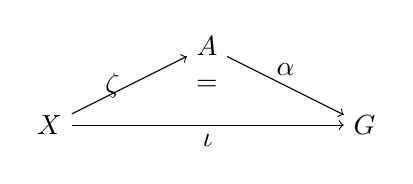
\begin{tikzpicture}
        \node (X) at (0,0) {\( X \)};
        \node (A) at (2,1) {\( A \)};
        \node (G) at (4,0) {\( G \)};
        \draw[ ->] (X) -- (A) node[midway, left] {\( \zeta \)};
        \draw[ ->] (X) -- (G) node[midway, below] {\( \iota \)};
        \draw[->] (A) -- (G) node[midway, above] {\( \alpha \)};
        \node at (2,0.5) {\( = \)};
    \end{tikzpicture}
\end{center}

The weight of the morphism \( \phi : G \to \mathcal{T}_\Sigma^X\) excluding morphisms in \( \Gamma' \) is defined as the number of morphisms from \( X \) to \( G \) that do not factor through any \( \alpha \in \Gamma \).

\begin{definition}[Weight excluding specific morphisms \cite{endrullis2023generalized}]
    \label{def:weight_excluding}
    The \textbf{weight of \( \phi \) excluding morphisms in \( \Gamma' \)} is defined as
    \[
        w_{\mathcal{T}_\Sigma^X}(\phi - \Gamma) \overset{\operatorname{def}}{=} \left| \operatorname{Hom}(X, G) \setminus \Gamma' \right|
    \]
\end{definition}

\begin{remark}
    If \( \Gamma \) is a singleton \( \{ \alpha \} \), we may simplify the notation by writing \( w_{\mathcal{T}_\Sigma^X}(\phi - \alpha) \) instead of \( w_{\mathcal{T}_\Sigma^X}(\phi - \{ \alpha \}) \).
\end{remark}
